\bigskip

Composition for quadraphonic installation, interpreted the 17th of June, 2019 at NOTAM in Oslo.

\bigskip

\noindent \textbf{{\large Presentation}}
\hrulefill

\bigskip

The composition \texttt{data-01} is a direct application of the work describe in the chapter \textsl{\nameref{am}} applied to a given sample defined as \texttt{data-01} and it is composed of 3 parts as layers.

\bigskip

\texttt{Can you imagine ...} 

\begin{itemize}[leftmargin=0.4in]
\item \textbf{Part I} : \textsc{Drop water as a Markov chain walk}. 

\texttt{... before the language ...} 

Interpreted as a continuum background, the part I is a Markov chain applied to the \textsl{Symbolisation} as \textsl{Hierarchical clustering} and the \textsl{Systemic analysis} as \textsl{Developmental process} of the referent sample.

\item \textbf{Part II} : \textsc{Collatz synthesis as a proportional canon}. 

\texttt{... and beyond the language ...} 

Triggered process, the part II is a proportional canon of a chosen rhythm (see figure \ref{rtm}) defined by the \textsl{Contrastive analysis} as \textsl{Segmentation by marker} of the sample. The Collatz algorithm as a normalized profile controls the bandwidth ratio of the \textsl{UGen} \texttt{Resonz} applied to a pink noise.

\item \textbf{Part III} : \textsc{Fractal on Radio}. 

\texttt{... and into the language.} 

Triggered process, the part III is a `fractalization' of the previous defined rhythm as an alternately spatialized streaming radio.

%\textbf{\textit{R\'ef.}} ...
 \end{itemize}

\smallskip

\noindent \textbf{{\large Synthesis}}
\hrulefill

\bigskip

\noindent  \textbf{
  %\textit{b/ } 
  Water drop }
  
\label{wd}

\smallskip

\begin{figure}[H]
\begin{center}
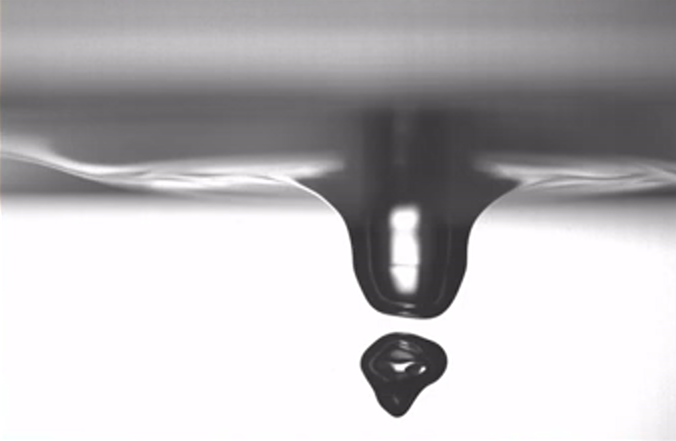
\includegraphics[width=0.65\linewidth]{img/3187} 
\caption{`The impact creates a cavity which then begins to recoil a small air bubble is then trapped under the water in a process referred to as bubble entrainment.' \citep{sdw}}
\label{dropwater}
\end{center}
\end{figure}

\noindent \textbf{
  %\textit{b/ } 
  Collatz resonance }

\label{colres}

\smallskip
This synthesis requires a Collatz sequence defined as follow:

\titlebox{\textit{\textbf{Collatz sequence}}}
{The Collatz sequence is a sequence of numbers relevant to the Collatz conjecture, which theorizes that any number using this algorithm will eventually be reduced to 1 or stop on the trivial cycle \texttt{(4 2 1)}.

Note that in this work, according to the range of number we might use, we are not concerned about this conjecture.

So, to get a Collatz sequence from any integer $n$ superior to 1, each step is depending of the previous such as if $n_i$ is even, divide $n_i$ by two to get $n_{i+1}$, and if $n_i$ is odd, multiply $n_i$ by three and add one to get $n_{i+1}$, until $n_{i+1}=1$. 
% The conjecture's truth is supported by calculations, but it hasn't yet been proved that no number can indefinitely stay above 1.
} 


The Collatz sequence is interpreted as a normalized profile -- see figure \ref{coltz} -- envelope which is defined by its duration as the length of the sequence according to a value of $dx$ in second. Note that the value zero is added at the end of the sequence.
\begin{lstlisting}[basicstyle=\footnotesize\ttfamily,language=Java]
Env.new(collatz.add(0).normalize, Array.fill(collatz.size, dx))
\end{lstlisting} 

%This envelope can be interpreted musically according to at least two \textit{modi operandi}.

%\begin{enumerate}
%  \item as $rq$
  
%  Then, this envelope set dynamically the value of the bandwidth ratio $rq$ (bandwidth/centerFreq) of a resonant filter, with the initial value of the Collatz sequence as the resonant frequency applied to a white noise.

This envelope is currently interpreted musically according to the value of the bandwidth ratio $rq$ (bandwidth/centerFreq) of a resonant filter.  Then, this normalized envelope set dynamically $rq$ with the initial value of the Collatz sequence as the resonant frequency applied to a pink noise.

\smallskip

\begin{algorithm}
\caption{$\sim$\textsc{collatz}$\,(n \,|\, r)$}\label{collatz}
\begin{algorithmic}%

\State \textbf{arg}
\State $\qquad n=$ integer
\State \textbf{arg -- recursive call}
\State $\qquad r=$ step result
\State

\If {$n$ is even}

$x=n/2$

\Else 

$x=3n+1$
\EndIf
\State
\If {$x \in r$} 

\Return $r$

\Else

$\sim$\textsc{collatz}($x,r.add[x]$)
\EndIf

\end{algorithmic}
\end{algorithm}

\begin{figure}[H]
\begin{center}
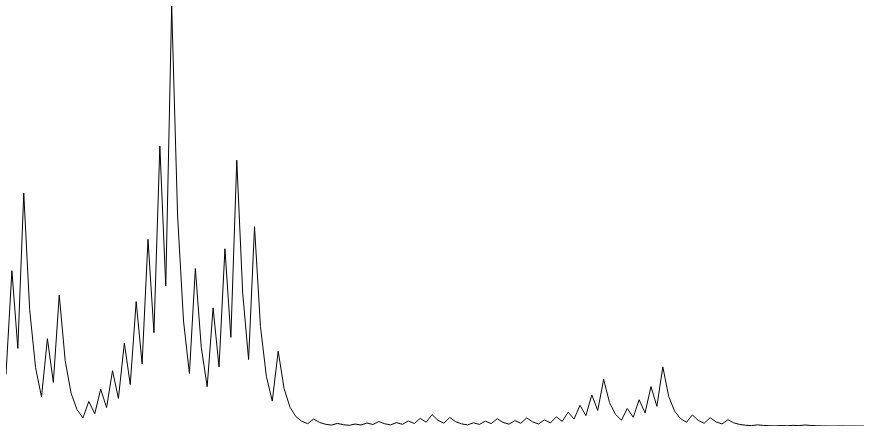
\includegraphics[scale=0.46]{img/8083.png}
\caption{Profile of the Collatz sequence started with the number 8083.}
\label{coltz}
\end{center}
\end{figure}

% This is more about experimental behavior of the algorithm \ref{coltz} $\sim$\textsc{collatz} as a volume envelope applied to the initial value as frequency. Then, the signal is the sum of all integers as frequencies of sinusoids, in a range between $1$ Hz to a given frequency as an integer. Each sinusoid is multiplied by its respective Collatz sequence as a volume envelope.

% The bias of this synthesis is about the computation of the signal which can takes a significative amout of time. Nevertheless, this approach allows as well as to think in terms of optimization than to reach at least the limit of the processor; and the result -- even if it cannot be used as such or in a real-time synthesis context -- remains an interesting listening as an experiment as well as a sound phenomenon than an algorithm processed directly on the signal and from scratch.

% For the record, I extended this principle for any array of frequencies as a list of integers. The relevance of this approach remains very relative, but this can be a guideline for further work -- see \nameref{cs} in Annex 3 p. \pageref{cs}.

%\newpage

\noindent \textbf{{\large Description}}
\hrulefill

\bigskip

  \textbf{
  %\textit{b/ } 
  Markov chain walk instantiation }
  
  \smallskip
 
 According to the Markov chain walk described in the section \textsl{\nameref{osc}} p. \pageref{osc}, 
 the values of the list to send -- done with the discriminative classification analysis of \textsl{enkode} -- according to durations as triggers \textit{in time}, are respectively the loudness as distance, the centroid and $f0$ as the frequencies drop variation interpreted as millimeter unit (see table p. \pageref{tab:apc}).
  
 \bigskip
\begin{lstlisting}[basicstyle=\footnotesize\ttfamily,language=Lisp]
;; Common Lisp Markov chain initialisation

N3> (defvar *DATA* (remove-duplicates (read-file "aaa.score")
   :test #'equalp))
N3> (create-mlt 'aaa (length (car *DATA*)) (length *DATA*)
   :carte #'rnd-map)
N3> (loop for neuron in (neurons-list aaa)
   for dat in *DATA* do (setf (output neuron) dat))
N3> (dendrogram aaa 3 :and-data t)
-6031.028+
N3> (open-graph *tree*)
N3> (defparameter *alpha-seq-9* (alpha-seq aaa *tree* 9))
*ALPHA-SEQ-9*
N3> (write-file (structure-s (list *alpha-seq-9*) :result :last) 
    :path "aaa.dat")
N3> (mk-alraw *alpha-seq-9* (read-file "aaa.raw"))
    min           max
0:  0.35861862    4.7338142
1:  1.8155038     4.197111
2:  260.4863      1782.7802
3:  1.6           1.6
4:  213.9862      2075.2625
\end{lstlisting}

\smallskip

\begin{lstlisting}[basicstyle=\footnotesize\ttfamily,language=Lisp]
;; the values to send are defined as follow:
(let ((nrand (random (length (car (getraw nep))))))
   (send-udp (read-from-string 
      (format nil "(\"/~A\" ~{\"~S\"~})"
         'N3
         (list
            (nth nrand (nth 1 (getraw nep))) ;f0
	    (nth nrand (nth 2 (getraw nep))) ;centroid
	    (nth nrand (nth 3 (getraw nep))) ;loudness
	  ))) 
      (string "127.0.0.1") 7771)
   (sleep (nth nrand (nth 0 (getraw nep)))))
\end{lstlisting}

\bigskip
\noindent Then, the incoming OSC message is interpreted in SuperCollider as follow:

\bigskip

\begin{tabular}{c|c|l}
\rowcolor{lightgray} \textit{Analysis}  & \textit{Parameter in SC}  & \multicolumn{1}{c}{\textit{Computation}}\\
%\hline
\textsl{duration} &  OSC trigger   & \multicolumn{1}{c}{none}  \\
\textsl{loudness} &  \texttt{dist}ance   &  \texttt{.linlin($min$, $max$, 0.6, 0.1)} \\
\textsl{centroid}, $f0$ &  \texttt{rad}ius 1 & \makecell{\texttt{rrand(}\textsl{centroid}, $f0$\texttt{)}\\ \texttt{.linexp($min$, $max$, 4, 1)}} \\
\end{tabular}
\label{tab:apc}

  \bigskip

 For convenience, the data needed for the Markov chain are stored in a \textsl{lisp} file. This concerns the \texttt{alpha-seq} according to the retained number of classes as \texttt{*alpha-seq-9*} and the hash table \texttt{*alraw*} which associates alpha symbol to all corresponding raw values.

%\bigskip
%\smallskip
\newpage
  
  \textbf{
  %\textit{b/ } 
  Proportional canon instantiation }
  
 % \smallskip
%(see  quantizers\cite{qmt} in N3) 

%...
\setlist[enumerate,1]{leftmargin=1.3cm}
\setenumerate{label*=\footnotesize {\textit {\arabic*.}}}
\begin{enumerate}
 \item Initiate some preliminary variables.

%\item[$\sim$score] -- generated with \textsl{enkode}, and defined with:
% \begin{lstlisting}[basicstyle=\footnotesize\ttfamily,language=Java]
%FileReader.readInterpret(".../enkode.data", true, true)
%.collect{|prm| prm.copyRange(0,4)
%.collect{|nn| nn.asFloat}};
%\end{lstlisting}

\textbf{$\sim$rtm} -- the selection of the rhythm \textbf{$\sim$rtm} is done inside to the panel of rhythm as indice according to the structure discrimination. The choice is done through a \textsl{pdf} file (see figure \ref{rtm}). 

\bigskip 

 \begin{figure}[htbp]
\begin{center}
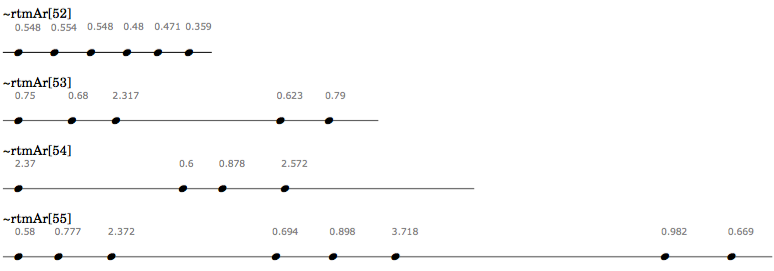
\includegraphics[scale=0.44]{img/6710} 
\caption{Extract of the list of rhythms generated with Lilypond as a \textsl{pdf} file.}
\label{rtm}
\end{center}
\end{figure}
 
This last is generated as follow:
 \begin{lstlisting}[basicstyle=\footnotesize\ttfamily,language=Lisp]
N3> (load (concatenate 'string *NEUROMUSE3-DIRECTORY* 
      "opt/lilypond.lisp"))
N3> (defparameter *seq-as-dur* 
  (loop for i in 
    (group-list (read-file "aaa.score") 
      (loop for i in (read-file "aaa.dat") collect 
        (car (mapcar #'(lambda (x) 
          (length (coerce (string x) 'list))) i)))) 
    collect 
      (loop for dur in (car (mat-trans i)) collect 
        (round (* 1000 dur)))))
*SEQ-AS-DUR*
N3> (write-rtm-seq *seq-as-dur* 
      :path "aaa.ly" 
      :title "data-01")
\end{lstlisting}
Then compile the Lilypond \textsl{aaa.ly} file.% in \textsl{src} folder.

\textbf{$\sim$repeat} -- number o repetition of \textbf{$\sim$rtm}.

\textbf{$\sim$duration} -- duration of the proportional canon.

\textbf{$\sim$ratio} -- currently the golden number.

\textbf{$\sim$numberOfVoices} -- currently 4 voices.

 \item Compute durations and delays.
\begin{lstlisting}[basicstyle=\footnotesize\ttfamily,language=Java]
~rrr = ~proportionalCanon.value(~numberOfVoices,~duration,
	~ratio,1);
 \end{lstlisting}
 \item Display for each event of each voice the timming, the associated score event and the voice number.
 \begin{lstlisting}[basicstyle=\footnotesize\ttfamily,language=Java]
~rrr = ~rrr.collect({|it,i|
	var a = (~rtm.flop[0].wrapExtend(~rtm.size*~repeat)
		.normalizeSum*it.first).addFirst(0);
	var b = a.copyToEnd(1);
	a.pop;
	[
		a.integrate+it.last,
		b,
		~rtm.wrapExtend(~rtm.size*~repeat),
		Array.fill(~rtm.size*~repeat, i+1)
	].flop
});
\end{lstlisting}

 \item Sort according to the timing for all voices.
  %\verbatimfont{\footnotesize}%
 \begin{lstlisting}[basicstyle=\footnotesize\ttfamily,language=Java]
~rrr = ~rrr.flatten(1).sort({ arg a, b; a[0] < b[0]});
\end{lstlisting}
 \item Add duration between two successive events.
 \begin{lstlisting}[basicstyle=\footnotesize\ttfamily,language=Java]
~rrr = [~rrr.flop[0].differentiate, ~rrr].flop;
\end{lstlisting}

%From this point, the following values are available according to the event \texttt{i} as: 
% \begin{itemize}
%\item[$$] \textsl{\textbf{duration}} $\rightarrow$ \texttt{$\sim$rrr[i][0]}
%\item[$$] \textsl{loudness} $\rightarrow$ \texttt{$\sim$rrr[i][1][2][1]}
%\item[$$] \textsl{\textbf{centroid}} $\rightarrow$ \texttt{$\sim$rrr[i][1][2][2]}
%\item[$$] \textsl{bass loudness} $\rightarrow$ \texttt{$\sim$rrr[i][1][2][3]}
%\item[$$] $\bm{f0} \rightarrow$ \texttt{$\sim$rrr[i][1][2][4]}
%\item[$$] \textsl{voice number} $\rightarrow$ \texttt{$\sim$rrr[i][1][3]}
% \end{itemize}
 
 \end{enumerate}
 
 %Or in other words, 
\noindent To complete the last point,  each event \texttt{i} as element of  \texttt{$\sim$rrr} is defined by the structure  \texttt{[a, [b, c, [d, e, f, g, h], i]]}  corresponding to:
 
  \begin{itemize}
\item[$ $] \texttt{a} $\rightarrow$ duration from the previous event until \underline{this} event, all voices combined (done in point \textit{5}.) $\Rightarrow$ \texttt{$\sim$rrr[i][0]};
\item[$ $] \texttt{b} $\rightarrow$ timeline of onset according to the total duration;
\item[$ $] \texttt{c} $\rightarrow$ duration of the event until the next event for \underline{this} voice;
\item[$ $] \texttt{d} $\rightarrow$ initial duration of  \texttt{$\sim$rtm};
\item[$ $] \texttt{e} $\rightarrow$ $f0$ $\Rightarrow$ \texttt{$\sim$rrr[i][1][2][1]};
\item[$ $] \texttt{f} $\rightarrow$ centroid $\Rightarrow$ \texttt{$\sim$rrr[i][1][2][2]};
\item[$ $] \texttt{g} $\rightarrow$ loudness;
\item[$ $] \texttt{h} $\rightarrow$ loudbass;
\item[$ $] \texttt{i} $\rightarrow$ voice number.
 \end{itemize}
 
 Note that the array \texttt{[d, e, f, g, h]} defines the event's parameters, which is computed  in this case with the command line \textsl{enkode}. 